\documentclass{article}
\usepackage{graphicx}
\usepackage{amssymb}
\usepackage{amsmath}

\begin{document}

\title{Robotics 811 - HW 2}
\author{Xiang Zhi Tan}

\maketitle

\section{Q1}
\section{Q2}
\subsection*{a}
Firstly, we calculate the values of $f(x_0),....f(x_i)$ which gives us the vector $0, 0.0434,
0.1269, 0.2217, 0.3187, 0.4145, 0.5075$. By plugging it in into the method with the following variables.
$dividedDifferences(6,2.25,xs,fxs)$. The method will return the result:$0.1737$ 
which is equal to the answer given by matlab which is $0.1737$.
\subsection*{b}
\begin{itemize}
	\item Using the procedure at $x=0.05$ with $n=2$, gave the estimate of $4.9878$.
	\item Using the procedure at $x=0.05$ with $n=4$, gave the estimate of $4.9442$
	\item Using the procedure at $x=0.05$ with $n=40$, gave the estimate of $4.5872$
\end{itemize}
The actual value of $f(0.05)$ is $4.5872$ which is same as the estimate of $4.5872$ by $n=40$
\subsection*{2(c)}
The Error estimate is as following:\\
\begin{tabular}{|c|c|}
\hline
$n$ & $E_n$ \\ \hline
2 & 3.4911\\
4 & 2.3584\\
6 & 3.5367\\
8 & 6.4873\\
10 & 12.9702\\
12 & 27.1445\\
14 & 58.4298\\
16 & 128.1824\\
18 & 285.0742\\
20 & 640.9705\\
40 & 2830400\\
\hline
\end{tabular}\\
The Error make sense, because we are trying to fit a polynomial on a non-polynomial function. As the interpolating polynomial will never become the function that we are trying to interpolating and it will only continue to over fitting the function causing massive error at the end of the functions
\section{Q3}
\section{Q4}
First we observe the graph of the function $x - tan(x) = 0$ around the 200 point to find good values to be tested. 
\begin{figure}[h]
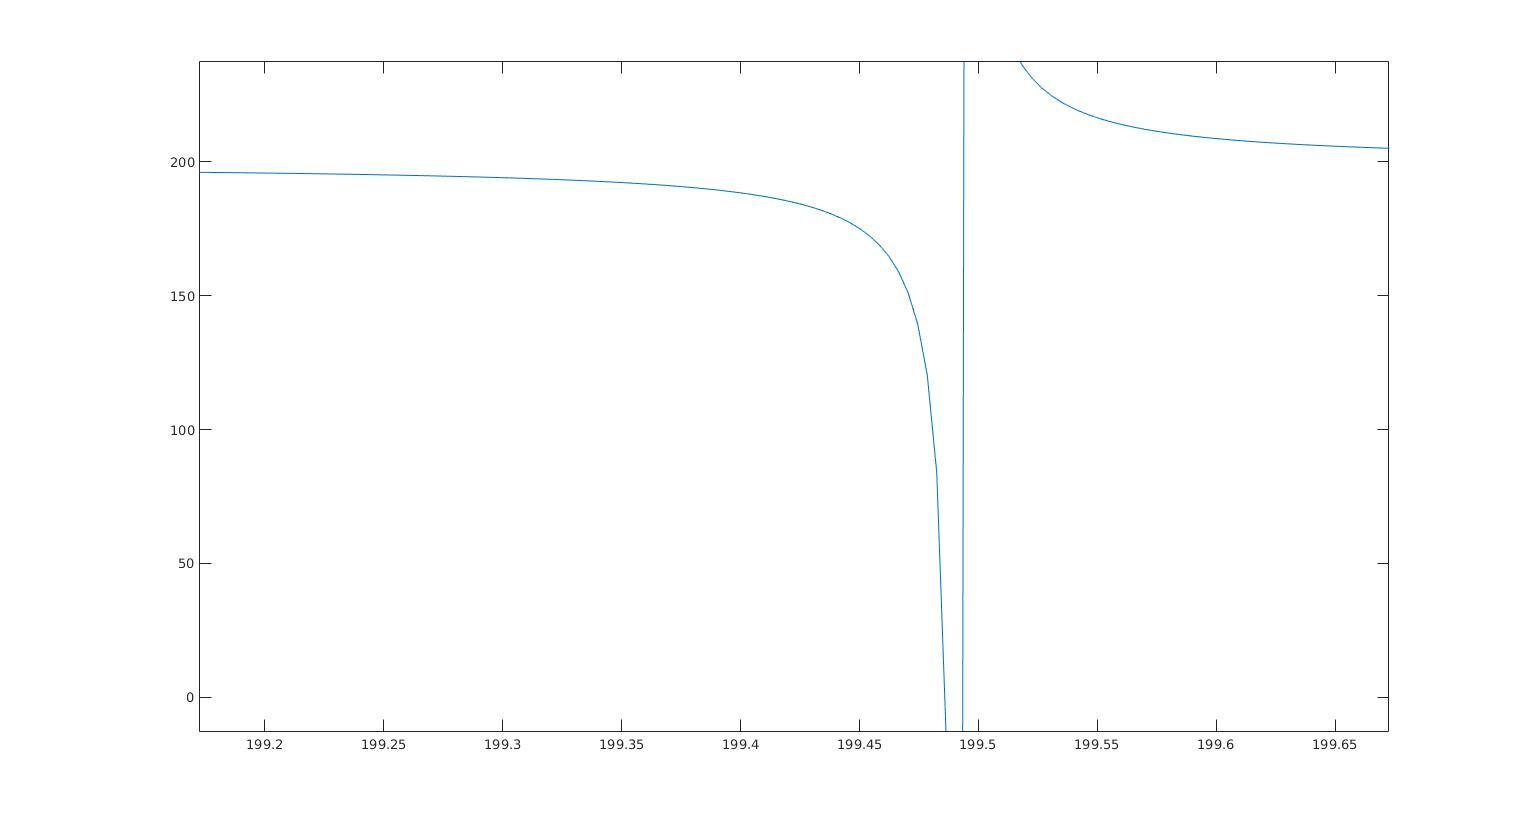
\includegraphics[width=4in]{p4.jpg}
\end{figure}\\
By visual inspection, we found that the root must be between $199.49$ and $199$. We tested this by inserting both values into the function and it gave us both $-682.7305$ and $197.1303$. Since $199.49$ won't be able to converge using Newton Method(implemented in the file titled \textit{newtonMethod.m}), we first use those two values in the bisection method to give an estimate root. The code for the function is attached to this paper under the title \textit{bisectionMethod.m}. The bisectionMethod returns $199.4861$ as the root. As we plugged in the value into newton method, it gave us the same value of $199.4861$. Therefore, the closet root to 200 is $199.4861$
\section{Q5}
\section{Q6}
\subsection{6(a)}
From the two polynomials given, we can construct a Sylvester's matrix:
\begin{equation*}
M = 
\begin{pmatrix}
1 &-12 &41 &-42& 0\\
0 &1   &-23 & 41 & -42\\
1& -2& -35& 0& 0\\
0& 0& 1& -2& -35\\ 
\end{pmatrix}
\end{equation*}
Calculating the determinant will give us
\begin{equation*}
det(M) = -7.1623e-12 \approx 0
\end{equation*}
Because the determinant is approximately 0, this means that $p(x)$ and $q(x)$ shares a common root.
\subsection{6(b)}
Using the ratio method discussed in class we constructed the following equation:
\begin{equation*}
\begin{aligned}
x &= \frac{x^4}{x^3} \\
&=(-1)^{1+2}\frac{det(M_1)}{det(M_2)} \\
&=(-1)\frac{
	\begin{vmatrix}
	-12 & 41 &-42 &  0\\
	  1 &-12 & 41 &-42\\
	 -2 &-35 &  0 &  0\\
	  1 & -2 &-35 &  0\\
	\end{vmatrix}
}{
	\begin{vmatrix}
	  1 & 41 &-42 &  0\\
	  0 &-12 & 41 &-42\\
	  1 &-35 &  0 &  0\\
	  0 & -2 &-35 &  0\\	
	\end{vmatrix}
}\\
&=(-1)\frac{806736}{-115248}\\
&=7
\end{aligned}
\end{equation*}
\section{Q7}
\subsection{7(a)}
\begin{figure}
\end{figure}
\subsection{7(b)}
\section{Q8}
\section{Q9}



\end{document}